%%================================================
%% Chapter 3
%%================================================
\chapter{การดําเนินงาน/วิธีวิจัย}
%\label{method}
\label{chapter3}

\section{ศึกษาการเขียนภาษา Go}
    ภาษาที่ใช้เขียน API นั้นมีหลากหลายภาษาไม่ว่าจะเป็น Python, Java, Kotlin หรือ Dart เป็นต้น โดยผู้จัดทำเลือกใช้ภาษา Go เนื่องจากขนาดและประเภทของงานตรงตามจุดประสงค์ที่สุดคือ การพัฒนา REST API และมี framework ที่เหมาะสมกับงานที่สุดนั่นคือ Gin framework ที่สร้างขึ้นมาเพื่อพัฒนา REST API โดยเฉพาะ

\subsection{หัวข้อที่เกี่ยวกับภาษา Go}

\subsubsection{ภาษา Go}
    ได้ทำการศึกษาการเขียน ภาษา Go\cite{Go} เพื่อนำมาสร้าง API เนื่องจากเป็นภาษาที่ได้รับความนิยมมากขึ้นเรื่อย ๆ ในยุคนี้โดยภาษา Go นั้นจะมีจุดเด่นในเรื่องของ Performance ที่\mbox{ทำงาน}ได้อย่างรวดเร็วเทียบกับภาษาอื่น ๆ อีกทั้งยังมีจุดเด่นคือความง่ายในการเขียนและการอ่าน และยัง\mbox{สามารถ}ทำ Concurrent Programming ได้ง่าย เพราะภาษา Go ถูกออกแบบมาเพื่อทำให้ Application ที่ต้องใช้ Multi-Threading หรือ Distributed Systems เป็นเรื่องที่ง่ายขึ้น
\subsubsection{Gin framework}
    หลังจากที่ได้ศึกษาหลากหลาย framework แล้ว ผู้จัดทำได้เลือกเป็น Gin framework\cite{Gin} เนื่องจาก Gin framework เป็น framework ที่ถูกสร้างขึ้นมาเพื่อ REST API และ มี feature หรือ libraries ที่สําคัญเหมาะกับ service ที่มีขนาดเล็กไม่มีความซับซ้อนมาก มีการแบ่งกลุ่ม API เพื่อความสะดวกในการใช้งาน
    
\section{ออกแบบ REST API ด้วยมาตรฐาน OAS}
OAS หรือ OpenAPI Specification เป็นมาตรฐานในการอธิบาย REST API ตัวหนึ่ง ๆ ที่สร้างมาเพื่อให้มนุษย์และคอมพิวเตอร์สามารถอ่านได้ โดยหลังจากเขียน OAS เสร็จสิ้น จะสามารถใช้เป็นแบบแผน เพื่อช่วยในการสร้าง พัฒนา และปรับปรุง REST API ให้ตรงกับ OAS ที่ได้ออกแบบไว้เพื่อการทํางานที่เป็นระบบและมีเป้าหมายที่ชัดเจน

\subsection{รูปแบบของ OpenAPI Specification}
        \begin{figure}[H]
            \centering
                \centering
                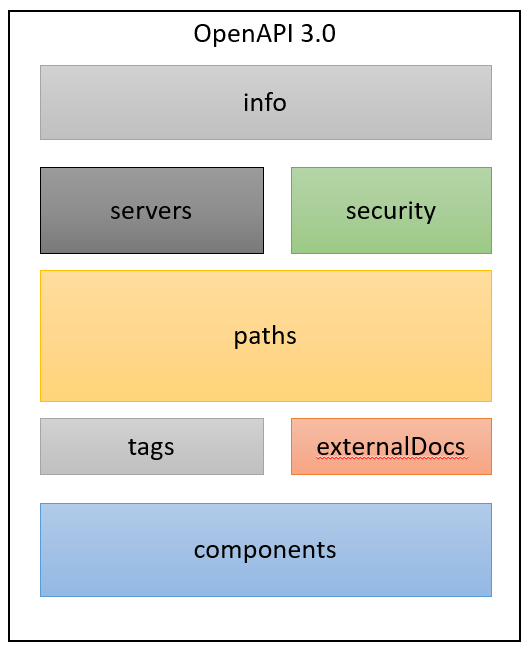
\includegraphics[width=5in]{latex/figures/openapi3.png}
            \captionsource{โครงสร้างของ OpenAPI}{\url{https://swagger.io/blog/api-design/openapi-driven-api-design/}}
        \end{figure}
จากโครงสร้าง OpenAPI ดังในรูปที่ 3.1 มีรายละเอียดดังนี้

\subsubsection{OpenAPI}
\raggedright ส่วนนี้จะเป็นการแสดงเวอร์ชันของ OpenAPI ที่ใช้ในการเขียน Specification ชุดนั้น ๆ
\subsubsection{Info}
\raggedright ส่วนนี้จะเป็นส่วนที่แสดงข้อมูลทั่วไปของ REST API คือ ชื่อ API, รายละเอียดเบื้องต้น, \mbox{ใบอนุญาติ} (license) ที่ใช้, ช่องทางการติดต่อ (contact) ของเจ้าของ API หรือ Terms of Service
\subsubsection{Servers}
\raggedright ส่วนนี้จะแสดงข้อมูลเกี่ยวกับเซิร์ฟเวอร์ที่ตั้งของ API
\subsubsection{Paths}
\raggedright ส่วนนี้เป็นส่วนที่ใหญ่ที่สุดใน Specification โดยเป็นส่วนที่แสดง Endpoint หรือ Path ต่าง ๆ ของ
API รวมถึง Operation ที่สามารถใช้กับ Endpoint นั้นได้ โดยในที่นี้ก็คือ HTTP verb ต่าง ๆ เช่น Get,
Post, Put, Delete เป็นต้น โดยในแต่ละ Path จะมีรายละเอียดดังนี้
     \begin{enumerate}
    \item รายชื่อกลุ่มที่มี Operation สามารถมีได้หลาย tag ใน Path เดียวกัน
    \item summary - ระบุความหมายและหน้าที่ของ Operation
    \item description - ระบุรายละเอียดการทํางานของ Operation
    \item operationId - เป็นค่า identity ของ Operation มักตั้งชื่อตรงกับชื่อฟังก์ชันในโค้ด เพื่อความสะดวกและป้องกันความสับสนเมื่ออ่านโค้ด
    \item security - ลักษณะของ Authentication ที่ต้องใช้ใน Operation นั้น
    \item requestBody - เป็นรายละเอียดของข้อมูลที่ต้องส่งมาให้ Operation ผ่านทาง RequestBody มักใช้ใน Operation ประเภท POST, PUT
    \item  parameters - สําหรับกําหนดรายละเอียดของข้อมูลที่ต้องส่งมาให้ Operation ทาง Query, Path, Header
    \item responses - สําหรับกําหนดรายละเอียดของข้อมูลที่ Operation จะทําการส่งกลับมาเมื่อทํางานเสร็จสิ้นแล้ว
\end{enumerate}

\subsubsection{Tags}
\raggedright ส่วนนี้เป็นส่วนไว้รวบรวมชื่อที่ใช้จัดกลุ่มของ Operation เพื่อให้สะดวกในการอ่านค่า response
\subsubsection{ExternalDocs}
\raggedright ส่วนนี้เป็นส่วนที่แสดง URL ของเว็บไซต์ที่มีข้อมูลนอกเหนือจาก Specification
\subsubsection{Components}
\raggedright ส่วนที่รวบรวมโครงสร้างต่าง ๆ เพื่อให้สามารถนําเฉพาะส่วน header ไปใช้ในส่วนอื่น ๆ ใน Specification
ได้ผ่านฟังก์ชัน reference

\subsection{การออกแบบ API ด้วยมาตรฐาน OpenAPI Specification}
หลังจากวางแผนรูปแบบของ REST API ที่ต้องการจะสร้างเสร็จสิ้นแล้ว ได้เริ่มทําการออกแบบ
OpenAPI Specification ผ่าน OpenAPI Editor Tool ที่มีชื่อว่า Stoplight Studio
\subsubsection{Stoplight Workspace}
    กําหนด Path จํานวน 2 Path คือ Path compile และ Path problem เพื่อเป็น
ตัวแทน API ทั้ง 2 ตัว หลังจากนั้นได้ทําการกําหนดรายละเอียดต่าง ๆ ภายใน Path ดังกล่าว ได้ออก
มาเป็นมาตรฐาน OpenAPI Specification โดยให้อยู่ในรูปของ YAML file format
        \begin{figure}[H]
            \centering
                \centering
                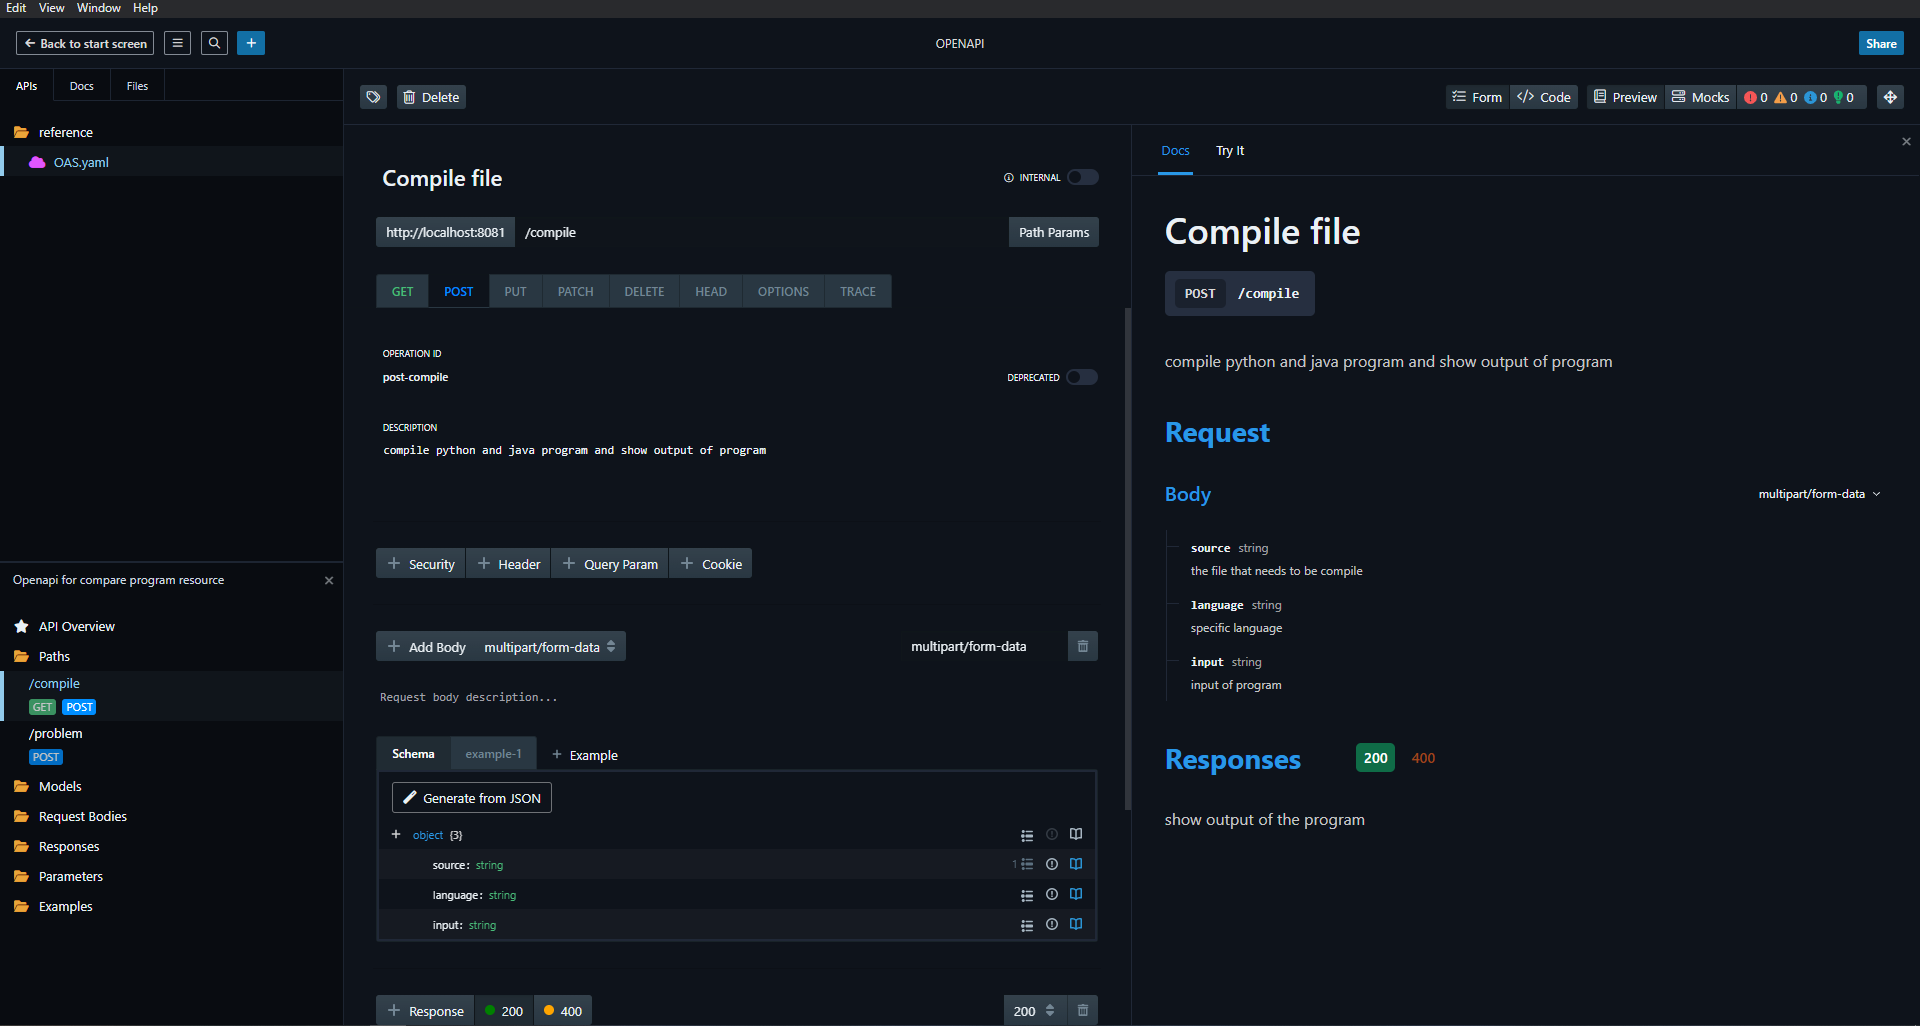
\includegraphics[width=5in]{latex/figures/stoplight.png}
            \caption{Stoplight Editor}
        \end{figure}
        \begin{figure}[H]
            \centering
                \centering
                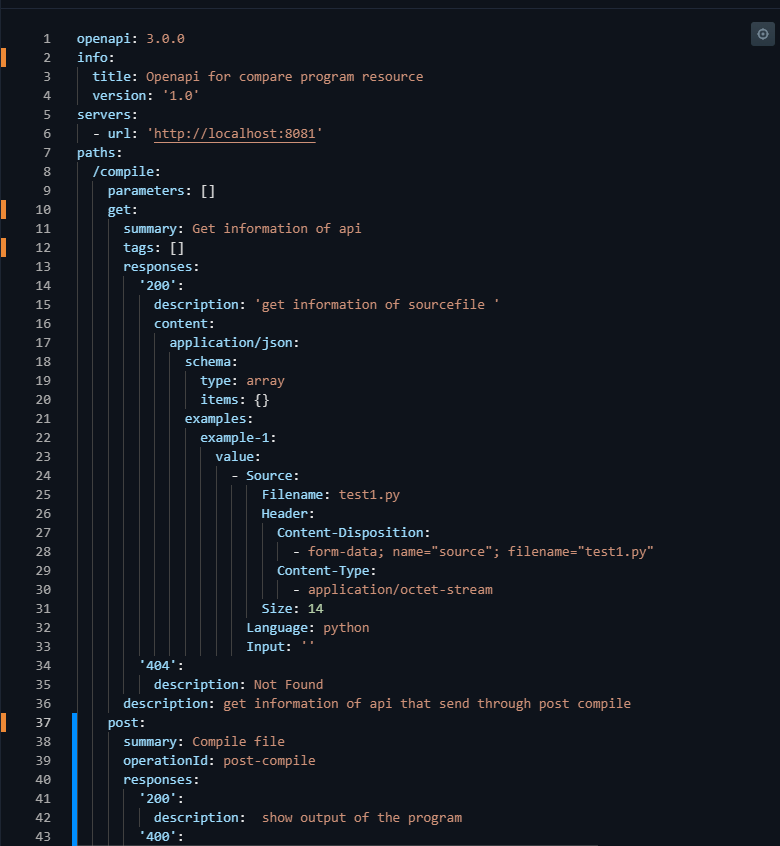
\includegraphics[width=5in]{latex/figures/OAS.png}
            \caption{OpenAPI Specification}
        \end{figure}

\section{การสร้างเอกสารประกอบ (API Documentation)}
หลังจากได้ออกแบบ API ตาม OAS เป็นไฟล์ในรูปแบบ YAML แล้ว จะเป็นการสร้างเอกสาร
ประกอบ หรือการสร้าง API Document กล่าวคือ เป็นเอกสารที่ช่วยให้การสื่อสารระหว่าง ส่วนการทํางาน
แบบด้านหน้า (Front-end) และด้านหลัง (Back-end) สามารถสื่อสารกันได้สะดวกมากยิ่งขึ้น โดยได้
เลือกใช้ OpenAPI Document Tool ที่มีชื่อว่า APITree ในการสร้างเอกสารประกอบดังกล่าว

        \begin{figure}[H]
            \centering
                \centering
                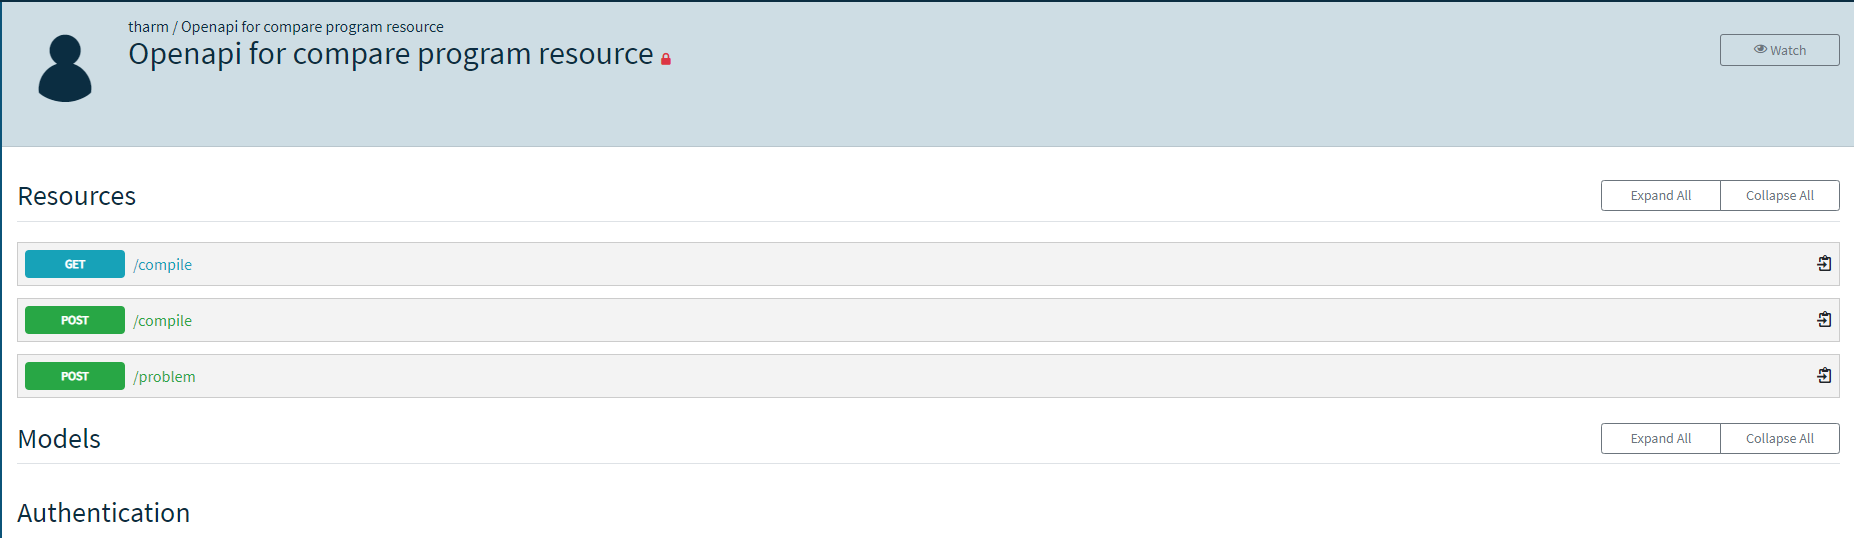
\includegraphics[width=5in]{latex/figures/apitree.png}
            \captionsource{APITree Document Page}{\url{https://hub.apitree.com/tharm/Openapi/}}
        \end{figure}
        \begin{figure}[H]
            \centering
                \centering
                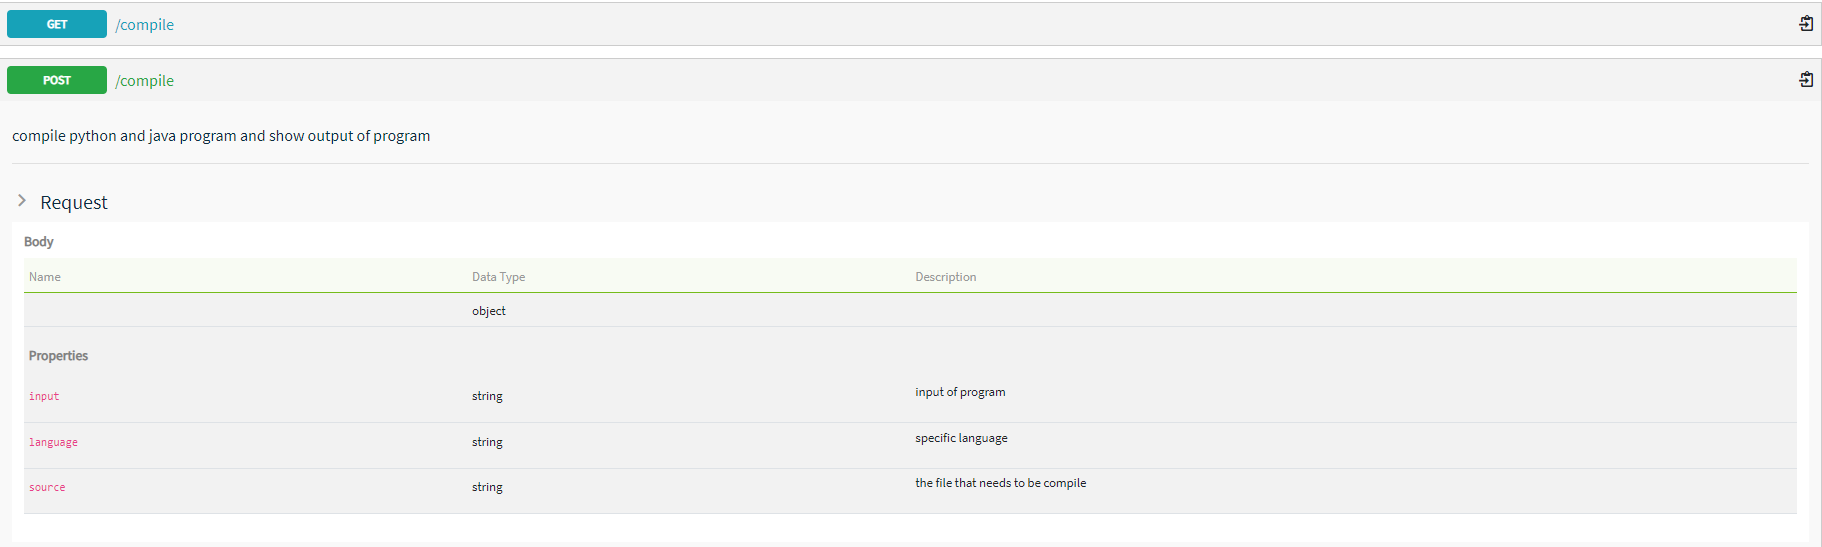
\includegraphics[width=5in]{latex/figures/apitree_detail.png}
            \captionsource{APITree Document Detail}{\url{https://hub.apitree.com/tharm/Openapi/}}
        \end{figure}
\section{การใช้งาน Docker Engine}
ในช่วงหลังของการพัฒนา ได้มีการนํา Docker \cite{docker} มาปรับใช้กับระบบการพัฒนา
ส่วนเบื้องหลัง โดยมีการสร้าง Docker image ขึ้นมาจากการเขียน Dockerfile และไฟล์ docker compose
\cite{compose} เพื่อให้ระบบ API สามารถทํางานได้บนคอมพิวเตอร์ทุกเครื่องที่ต้องการ และมีความสะดวกและ
รวดเร็ว ซึ่งเป็นคุณสมบัติเด่นของ Docker engine

